\subsection{Camera Operation}
Several important criteria were analyzed in order to find a proper camera module for this project. After selecting a  camera for use, further research was then performed to determine how the chosen module was operated. 
\subsubsection{Camera Selection}  \label{camdecision}
Due to our limited project budget of \$250, we focused on finding camera modules that were low-cost and simple to communicate with. This ruled out many low-cost camera modules that relied on complicated communications protocols, as well as all commercially available stereo image sensor suites. One other important factor that we sought to satisfy in our camera setup was the use of global shutter cameras, which acquire image data from the entire image sensor at once, rather than sequentially by pixel. The use of global shutter camera modules made it so that our setup was not susceptible to lens artifacts, or distorted imagery due to moving objects or a moving camera setup. With these factors kept in mind, the decision matrix shown below was created for selecting a proper camera module. Each module evaluated was given a ranking from 1-10 based on several categories, with 10 representing the ideal camera module for our project. 
\par
\singlespacing
\begin{small}
\centerline{
\begin{tabular}{ |L{2cm}|L{1.5cm}|L{2.5cm}|L{1cm}|L{1.7cm}|L{2cm}|L{1.7cm}|L{1.2cm}|L{1cm}| } 
 \hline
 \textbf{Camera Module} & \textbf{Max Frame Rate (FPS)}  & \textbf{Resolution at Max Frame Rate (px.)} & \textbf{Cost} & \textbf{Requires External Adapter} & \textbf{Data Transfer Interface} & \textbf{Shutter} & \textbf{Field of View (deg.)} & \textbf{Rank 1-10}  \\ \hline
 OV7670 & \cellcolor{red!25} 30 & \cellcolor{green!25} 640x480 & \cellcolor{green!50} \$10 & \cellcolor{green!25} No & \cellcolor{green!25} Parallel & \cellcolor{red!25} Rolling & \cellcolor{red!25}  25 & 5  \\ \hline
 Raspberry Pi Camera &\cellcolor{green!25}  90 & \cellcolor{green!25} 640x480 & \cellcolor{green!25}  \$30 & \cellcolor{red!25} Yes, \$53 & \cellcolor{red!25} MIPI (CSI2) & \cellcolor{red!25}  Rolling & \cellcolor{green!25} 49 & 6  \\  \hline
 PC1089K & \cellcolor{green!25} 60 & \cellcolor{green!25} 720x480 & \cellcolor{green!25} \$32 & \cellcolor{green!25} No & \cellcolor{red!50} NSTC/ PAL & \cellcolor{red!25} Rolling & Not Given & 5 \\ \hline 
 OV4682 & \cellcolor{green!50} 330 & \cellcolor{green!25} 640x480 & \cellcolor{red!25} \$89 & \cellcolor{red!25} Yes, \$50 & \cellcolor{red!25} MIPI & \cellcolor{red!25} Rolling & Not Given & 6 \\ \hline
 \textbf{MT9V034} & \cellcolor{green!25} \textbf{60} & \cellcolor{green!25} \textbf{752x480} & \cellcolor{red!25} \textbf{\$73} & \cellcolor{green!25} \textbf{No} & \cellcolor{green!25} \textbf{Parallel} & \cellcolor{green!50} \textbf{Global} & \cellcolor{green!25} \textbf{55} & \textbf{9} \\ \hline   
\end{tabular} }
\end{small}
\vspace{0.5cm}
\doublespacing
\par
Based on our decision matrix, we believed that the MT9V034 camera module was ideal for our stereo camera interface. These camera modules were the only low-cost global shutter option we were able to find in our research. Global shutter cameras contain specialized circuitry for acquiring image data from all pixels simultaneously, thus reducing motion-based artifacts and making them ideal for taking images in a sensor suite that is susceptible to motion. The MT9V034 also used a parallel data interface and relied on an external clock and shutter trigger, which made the module ideal for interfacing with an FPGA-based stereo imaging setup. 
\par
After obtaining two of the MT9V034 cameras, the operation of the camera modules was then investigated. In order to gather working images from each camera module, we began by reverse engineering the camera module breakout boards purchased. The MT9V034 camera breakouts used were purchased through Leopard Imaging Inc. Although these camera module breakout boards were intended to be used with Leopard Imaging's LeopardBoard ARM development board, the breakouts were found to contain only the supporting circuitry recommended in the MT9V034 datasheet, and we decided that they were ideal for our application \cite{livm34lp,mt9v034}. Once the schematics of each camera module breakout were known, a basic control interface for each camera was then designed.
\subsubsection{Camera Signaling}
By default, the MT9V034 camera module continuously gathered image data at 60Hz while supplied with an external clock signal and output enable signal \cite{mt9v034}. In this operating mode, several output signals from the camera module were used to transmit image data. Each image, or frame, was broken up into individual "lines" which corresponded to a line of pixels that stretched the width of the frame. Since our camera module captured images at 752x480 pixel resolution, one frame contained 480 lines of 752 pixels each. The camera modules broke up image data by frame and line, and camera data pins FRAME\_VALID and LINE\_VALID were toggled to indicate the transmission of a frame or line. The timing diagram shown in Figure \ref{FvLv} shows the operation of these pins while transmitting an image.

\begin{figure}[H]
	\centerline{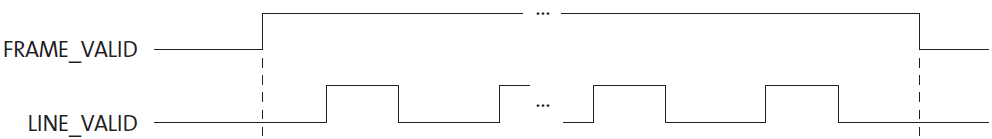
\includegraphics[width=1.0\textwidth]{camFvLv.png}}
	\caption{Frame and Line Valid \cite{mt9v034}}
	\label{FvLv}
\end{figure}

\par
Since the MT9V034 camera module transmitted pixel data in parallel and each pixel contained 10 bits of resolution, 10 pins were used to transmit pixel values. Pixel data was transmitted in correspondence with LINE\_VALID and output clock signal PIXCLK. When LINE\_VALID was asserted, the pixel data pins were updated with values corresponding to pixels 0-751 of the given line. Values for each pixel were written out on the falling edge of the camera's PIXCLK pin, which allowed for pixel values to be read on each rising PIXCLK edge. A full LINE\_VALID data transmission sequence therefore contained 752 PIXCLK cycles, which corresponded to the 752 pixels that made up the given line. A timing diagram of this data transmission scheme is shown in Figure \ref{LvDout}.  
\begin{figure}[H]
	\centerline{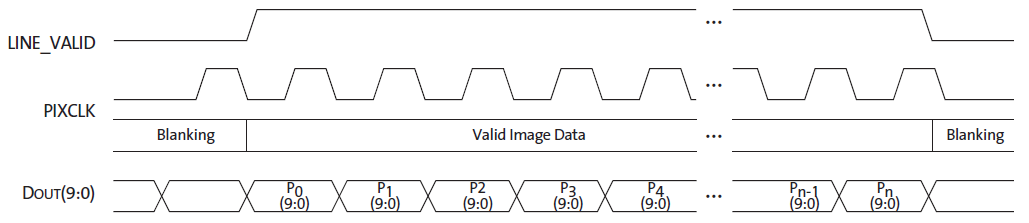
\includegraphics[width=1.0\textwidth]{camLvPckDout.png}}
	\caption{Line Data Transfer \cite{mt9v034}}
	\label{LvDout}
\end{figure}

\par
The default camera data transmission scheme was also examined using an oscilloscope, as shown in Figure \ref{camDataTransfer}, with channels 1-4 corresponding to camera PCLK, FRAME\_VALID, LINE\_VALID, and Data[0], respectively. In the case of Figure \ref{camDataTransfer}, the camera was initially powered off, resulting in an inactive PCLK signal during the beginning of the recording.
\begin{figure}[H]
	\centerline{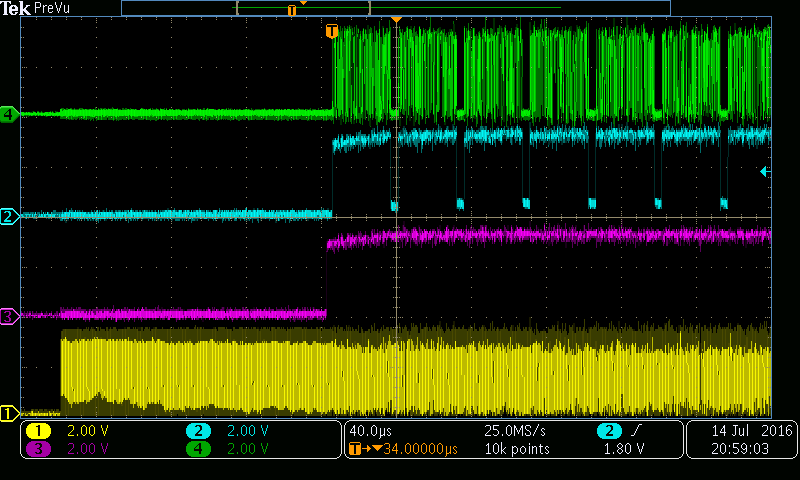
\includegraphics[width=1.0\textwidth]{oScope/pclk_fv_lv_data2/tek00004.png}}
	\caption{Camera Data Transfer}
	\label{camDataTransfer}
\end{figure}

\subsubsection{I$^2$C Control} \label{cameraI2Cdescription}
The MT9V034 Camera module's mode of operation was configured using a standard I$^2$C control interface. I$^2$C, or Inter-Integrated Circuit, is a bidirectional serial interface that allows for a master device to read from and write to several slave devices sharing the same data bus. The I$^2$C interface used contained a Serial Data Line (SDA) and Serial Clock Line (SCL) that were normally pulled to 5V. When one connected I$^2$C device wished to communicate with another, it pulled the SDA line low while leaving the SCL line high. The master device then began clocking the SCL line, and SDA was used to transfer 7 bits representing the address of the desired slave device, along with an 8th bit that represented whether a read or write operation was being performed. An example of this transfer is shown in Figure \ref{I2Cexample}. After this initial transfer, a second 8 bit sequence representing a specific register within the slave device was then transmitted. 
\par
As an example, if the master device wished to write to slave device 0x40 at register 0x00, it transmitted 0x41 (address 0x40 and WRITE), followed by 0x00. If the slave device received this transmission, it acknowledged by pulling the SDA line low. If this acknowledgement was successfully delivered, the master then transmitted the value that it wished to write to the given slave address and register. If the operation was a read rather than a write, the slave then transmitted a value back to the master.  
\par
\begin{figure}[H]
	\centerline{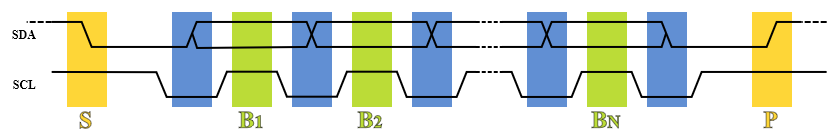
\includegraphics[width=1.0\textwidth]{I2C_data_transfer.png}}
	\caption{Example I$^2$C Data Transfer}
	\label{I2Cexample}
\end{figure}

Based on the LIVM34LP camera board schematic, each breakout board was configured so that its camera module was accessible at I$^2$C address 0x58 \cite{livm34lp,mt9v034}. Note that since both cameras came configured with the same I$^2$C bus address, a pullup resistor needed to be added to one of the cameras I$^2$C address lines so that both were individually accessible on a shared bus.

\subsubsection{Image Buffering}
Since each camera image contained 752x480 pixels with 10 bits of resolution per pixel, a full camera image consumed 3,609,600 bits, or 440.6kB, as shown in Equation \ref{imagesize}.
\begin{equation} \label{imagesize}
\textrm{Image Size} = 752px*480px*10\frac{bits}{pixel} = 3609600\,bits*\frac{1\,byte}{8\,bits}*\frac{1 kB}{1024\,bytes} = 440.625kB
\end{equation}
\par
In order to send a camera image to a computer or monitor for viewing, several steps needed to be taken. Although it would have been ideal to transfer the image directly from the camera to a computer or display, this was difficult to achieve due to the high speeds of the camera's data output. In order to properly synchronize camera data with a VGA display, both the camera and VGA display needed to run at exactly the same clock speed. The same amount of vertical and horizontal blanking was also required to display each pixel in its correct location. If the image was transferred to a computer, the act of packaging the information so that it was interpreted by said computer would  have placed severe limitations on the speed of the system. A proper solution to these timing issues was to buffer image data between the camera and the desired output source, which allowed for separate clock domains to be used for camera data transfer and data output. However, the act of locally buffering a camera image on an FPGA was difficult due to low memory resources. 
\par
Although 440kB seemed like a relatively small image size, creating a buffer object large enough for storing said image would have consumed an extremely large amount of FPGA resources. For reference, the Nexys3 FPGA evaluation board initially used for camera testing contained only 18kB of onboard Block RAM, and was not able to buffer an image of this size without the use of external memory\footnote{Xilinx, \textit{Spartan-6 FPGA Block RAM Resources}, 11.\\  \url{http://www.xilinx.com/support/documentation/user_guides/ug383.pdf}}. This left the final option of using either external memory or a First-In First-Out (FIFO) memory array for transferring a captured image between clock domains. 
\par
During initial development, an AL422B FIFO IC was used, since the IC was created specifically for buffering VGA imagery similar to that of the MT9V034 camera module, and was able to connect directly to the camera module data output lines \cite{al422b}. The AL422B FIFO module contained 3M-bits of RAM that were written to and read from in parallel, and supported separate input and output clock speeds between 1-50MHz \cite{al422b}. This meant that the camera module was able to write pixel data to the FIFO as long as it operated at a speed between 1 and 50MHz, and the FPGA was able to independently read from the FIFO at any speed within the same range. Note that since this FIFO supported only 8-bits of parallel data input and output, the lowest two bits of camera pixel data were truncated. This was not a major issue, since the truncation corresponded to a 4/1024 reduction in the range of values that each pixel mapped to.